\chapter{Análise Bibliográfica sobre Malware, por Gabriel dos Santos Martins\label{chap:bibliometria:gsmartins96}}

\section{Planejamento do estudo}

Com o avanço da tecnologias novas ferramentas e sistemas para facilitar tarefas diárias vem aparecendo e cada vez mais ganhando espaço no nosso dia a dia, tornando algo comum e de fácil acesso. Assim como na vida real sempre existe pessoas querendo ganhar dinheiro fácil de forma ilícita e na internet não é diferente, também existem pessoas má intencionadas procurando formas de prejudicar os outros e ganhar algum dinheiro em cima disso através de softwares maliciosos ou também conhecido como \textit{Malware}. 

Em dispositivos moveis o \textit{Malware} é identificado em aplicativos que invadem a privacidade do usuários roubando dados de seu aparelho através de \textit{APIs} do sistema {Android} como acessar os contados, arquivos, rede interna, etc.

Dessa forma várias pessoas já tiveram seu celular invadido e teve seus dados roubados ou espalhados na internet não só através de aplicativos mas acessando e-mails, sites com propagandas enganosas e diversas outras maneiras pela web. Os \textit{malware}s então vem se tornando cada vez mais comum e os estudos para combater e diminuir as vitimas infectadas por \textit{malware} tornam-se cada vez mais comum e debatido no meio de segurança da informação e pelos próprios desenvolvedores de \textit{software} e pela web com o intuito de conscientizar as pessoas a se atentarem no momento de realizar algumas ações na internet.

Software ilícitos além de roubar dados dos usuários e invadir a privacidade dos mesmo, também é utilizado para danificar dispositivos bloqueando o acesso a eles em troca de uma quantia em dinheiro para liberação, ação essa que acontece em grandes organizações e tomam conta da mídia reportando tal ocorrido. 

Partindo dos pontos acima, as questões que nortearam a pesquisa foram:
\begin{itemize}
    \item Quais técnicas mais utilizadas para detecção de \textit{malware}?
    \item Quais as formas mais comum de se infectar por \textit{malware}?
    \item Já existem ferramentas eficazes para detecção e combate a \textit{softwares ilícitos}?
\end{itemize}

\subsection{Uso do Bibliometrix e Biblioshiny}
Serão usadas a ferramenta e o \textit{workflow} proposto pelos autores do pacote Bibliometrix, conforme indica a figura ~\ref{fig:bibliometrix:workflow}.

\subsection{Limitações} O exercício relatado foi feito em 7:30 horas, utilizando a base de dados Web of Science (WoS) com auxilio do R/RStudio e a da ferramenta do RStudio Bibliometrix para as análises feitas geração dos gráficos apresentados aqui. 

\section{Coleta de dados\label{MASSA:coleta}}

A coleta de dados feita usando a base Web of Science (WoS) no dia 08 de janeiro de 2022, acessado por meio do Portal de Periódicos da CAPES.

As buscas formam feitas nas coleções \textbf{Science  Citation  Index  Expanded (SCI -EXPANDED)} e \textbf{Social  Sciences  Citation  Index (SSCI)}, que contém registros relativos a vários campos do conhecimento, no qual o SCI-EXPANDED foca mais na área das ciências exatas e naturais, enquanto que o SSCI indexa artigos da área das ciências sociais. Observe que os artigos nessas duas coleções são indexados desde 1945. 

Foi usada a \textit{query} de busca ilustrada na listagem:

\lstinputlisting[numbers=left,basicstyle=\normalsize\ttfamily,caption={Query de busca sobre Deepfakes.}]
{experiments/gsmartins96/AnaliseBibliometrica/Malware/query.txt}

\subsection{Explicação para os termos de busca usados\label{sec:titofrota:query}}

A busca utilizou palavras chaves que retornassem registros relacionados a \textit{malwares} no geral e que se relacionassem ao mesmo tempo com \textit{softwares ilicitos} e aplicativos \textit{android}, como sendo um dos mais afetados por \textit{malware} nos últimos anos. 

Os termos \texttt{malwares}, \texttt{software} e \texttt{malicious} buscam resultados sobre \textit{malwares} relacionados a sistemas que acessam a internet no geral, englobando todo tipo de software que contenha algo malicioso em seu funcionamento.

Foram obtidos 6,578 registros com a \textit{query} utilizada, porém a exportação foi feita apenas com 1000 desses registros com todos os 29 campos disponíveis junto.

\section{Análise dos dados}

\begin{figure}
    \centering
    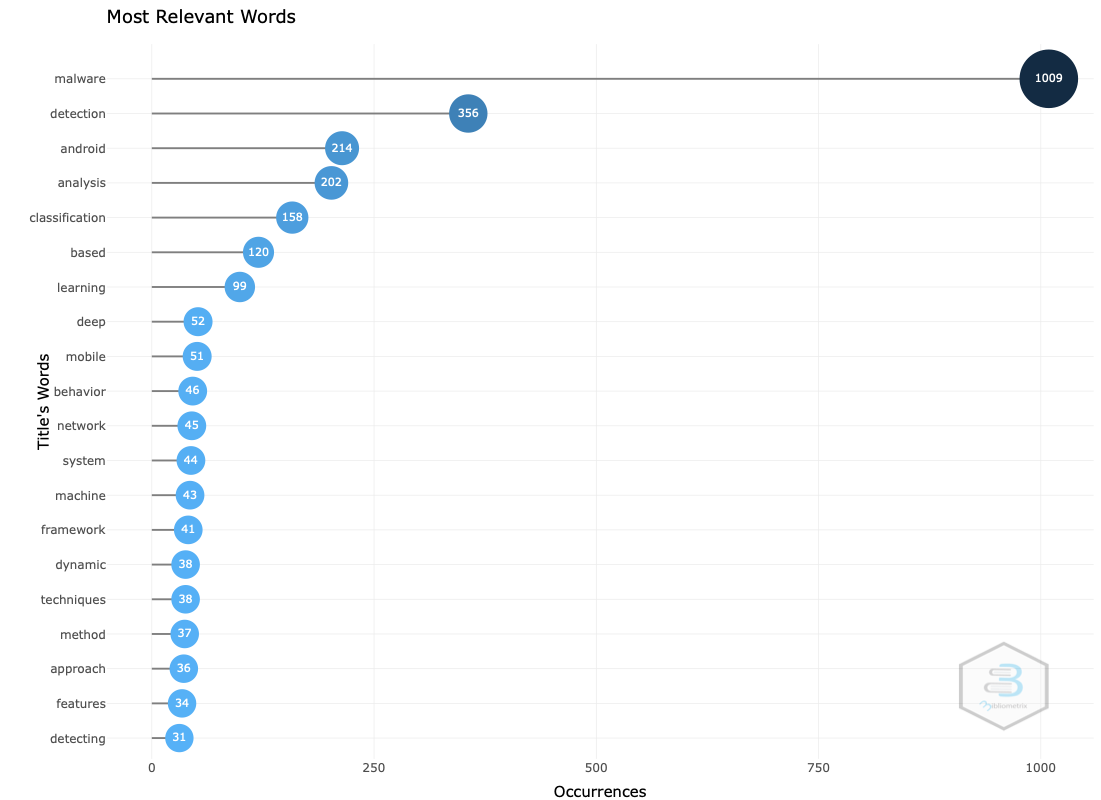
\includegraphics[width=1\textwidth]{experiments/gsmartins96/AnaliseBibliometrica/Malware/Figs/most-relevant_words.png}
    \caption{Palavras mais usadas \textit{dataset}}
    \label{fig:MALWARES@gsmartins96:MostUsedWords}
\end{figure}

A figura \ref{fig:MALWARES@gsmartins96:MostUsedWords} mostra as palavras mais relevantes utilizadas na pesquisa o que faz aumentar nossa compreensão sobre o tema e sobre a análise dos dados feita.

\subsection{Filtragem de registros}

Para a filtragem, foi removido alguns registros que não seriam úteis para a análise bibliométrica. O objetivo era apena estudos relacionados a malwares e softwares maliciosos que continham informações cientificas e estudos relacionados, sendo assim foi excluído criticas, resumos e etc. Com a aplicação do filtro apenas 423 registros foram mantidos e que servirá como objeto de análise.

\subsection{Análise descritiva do \textit{dataset} }

As informações mais gerais sobre o \textit{dataset} são as seguintes:
\begin{description}
    \item [\textit{Timespan}] Os artigos filtrados foram publicados entre 2005 e 2021, o que indica que quando a internet começou a crescer, os primeiros casos de malwares começaram a surgir.
    \item [\textit{Sources (Journals, Books, etc)}] Houve um pico de publicação de artigos no ano de 2019, com 135 documentos publicados.
    \item [\textit{Average years from publication}] A média do tempo de publicação dos artigos no \textit{dataset} é de 5,47 anos.
    \item [\textit{Average citations per documents}] Cada artigo no \textit{dataset} foi citado, em média 11,47 vezes.
    \item [\textit{Average citations per year per doc}] Após publicado, cada um dos artigos foi citado, em média, 1,649 vezes por ano.
    \item [\textit{References}] O \textit{dataset} contém 17.357 referências citadas.
    \item [\textit{Keywords Plus (ID)}] 203 distintas palavras-chave do tipo Keywords Plus (ID) foram encontradas no \textit{dataset}.
    \item [\textit{Author's Keywords (DE)}] 1812 distintas palavras-chave indicadas pelos autores foram encontradas no \textit{dataset} .
    \item [\textit{Author Appearances}] Os 3.640 distintos (nomes de) autores foram encontrados 2.297 vezes, como autores de artigos.
    \item [\textit{Authors of single-authored documents}] Dentre os 3.640 distintos (nomes de) autores encontrados, 28 deles editaram artigos individualmente, isso é, sem co-autores.
    \item [\textit{Authors of multi-authored documents}] Dentre os 3.640 distintos (nomes de) autores encontrados, 2.615 deles editaram artigos com um ou mais co-autores"
    \item [\textit{Single-authored documents}] Dentre os 994 documentos presentes no \textit{dataset}, 31 foram escritos por um único autor, e os restantes foram elaborados em co-autoria.
    \item [\textit{Documents per Author}] Dentre os 3.640 distintos (nomes de) autores, cada um publicou em média 0,376 artigos.
    \item [\textit{Authors per Document}] Cada um dos 994 documentos presentes no \textit{dataset} foi autorado com 2,66 autores em média.
    \item [\textit{Co-Authors per Documents}] As 2.615 aparições de (nomes de) autores (``Author Appearances''), sem distribuem, em média 3,66.
\end{description}

\subsection{Evolução da Produção Científica}

\begin{figure}
    \centering
    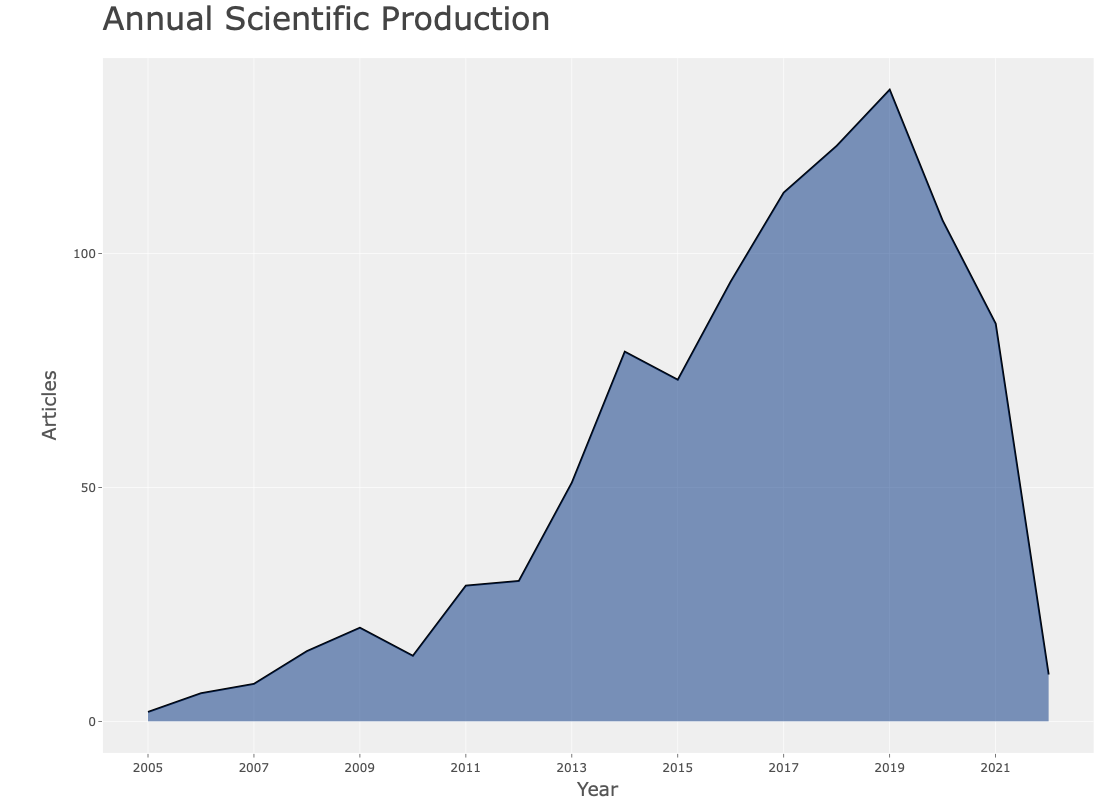
\includegraphics[width=1\textwidth]{experiments/gsmartins96/AnaliseBibliometrica/Malware/Figs/annual_scientific_production.png}
    \caption{Evolução da produção científica no \textit{dataset}}
    \label{fig:evol:anual:MALWARES@gsmartins96}
\end{figure}

A figura \ref{fig:evol:anual:MALWARES@gsmartins96} representa a revolução em produção cientifica mundial a respeito do tema. Houve um grande pico no ano de 2019 e os primeiros surgimentos de artigos no ano de 2005.

\subsection{Interpretação do Crescimento}

O crescimento nos últimos anos e o notável pico que teve em 2019 de acordo com o \textit{dataset} demonstra que o tema tem chamado muita atenção a medida que a tecnologia evolui em decorrência da grande quantidade de dados que temos armazenados na nuuvem e em nossos aparelhos celulares, como forma de proteger essas informações sigilosas de pessoas má intencionadas.

\subsection{Evolução das Citações}

\begin{figure}
    \centering
    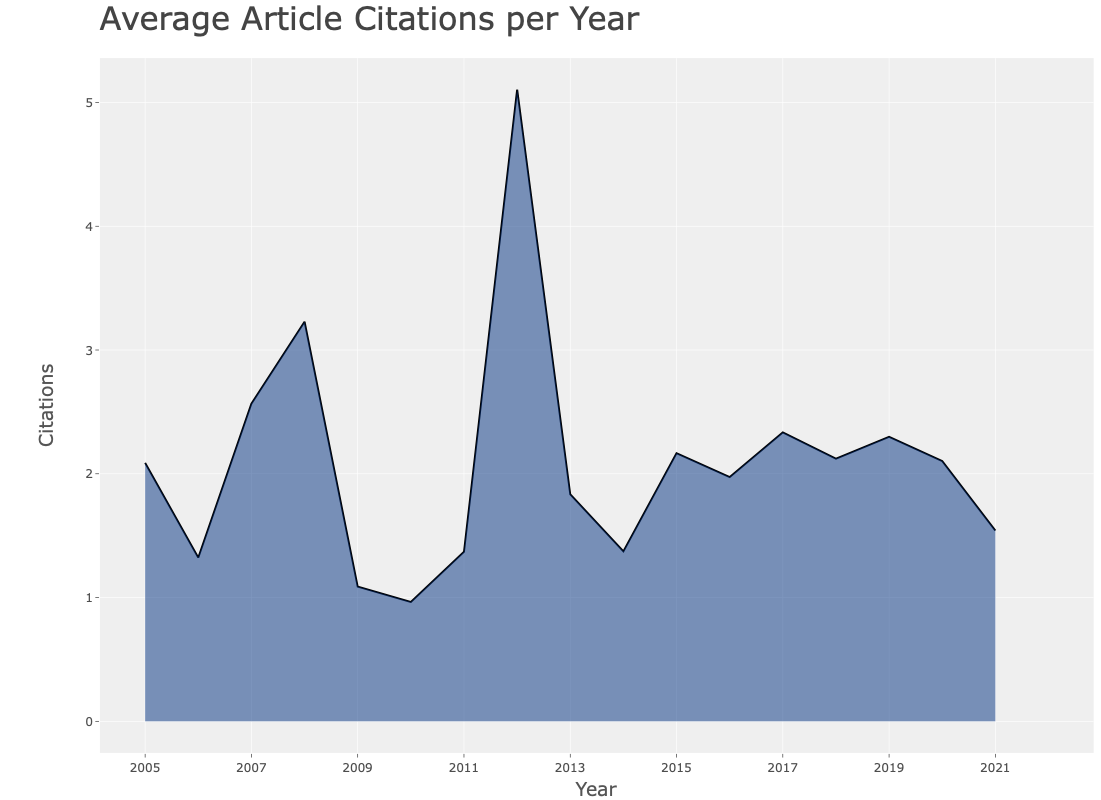
\includegraphics[width=1\textwidth]{experiments/gsmartins96/AnaliseBibliometrica/Malware/Figs/citations_per_year.png}
    \caption{Evolução da produção científica no \textit{dataset}}
    \label{fig:evol:anual:citations:MALWARES@gsmartins96}
\end{figure}

A figura \ref{fig:evol:anual:citations:MALWARES@gsmartins96} apresenta a evolução das citações aos artigos do \textit{dataset} demonstrando um pico em 2013 onde começaram a surgir mais \textit{sistemas web} e \textit{aplicativos} e no decorrer dos anos vem mantendo uma media de 2 citações por ano

\subsection{\textit{Three-Field Plots (Sankey diagram)}}

\begin{figure}
    \centering
    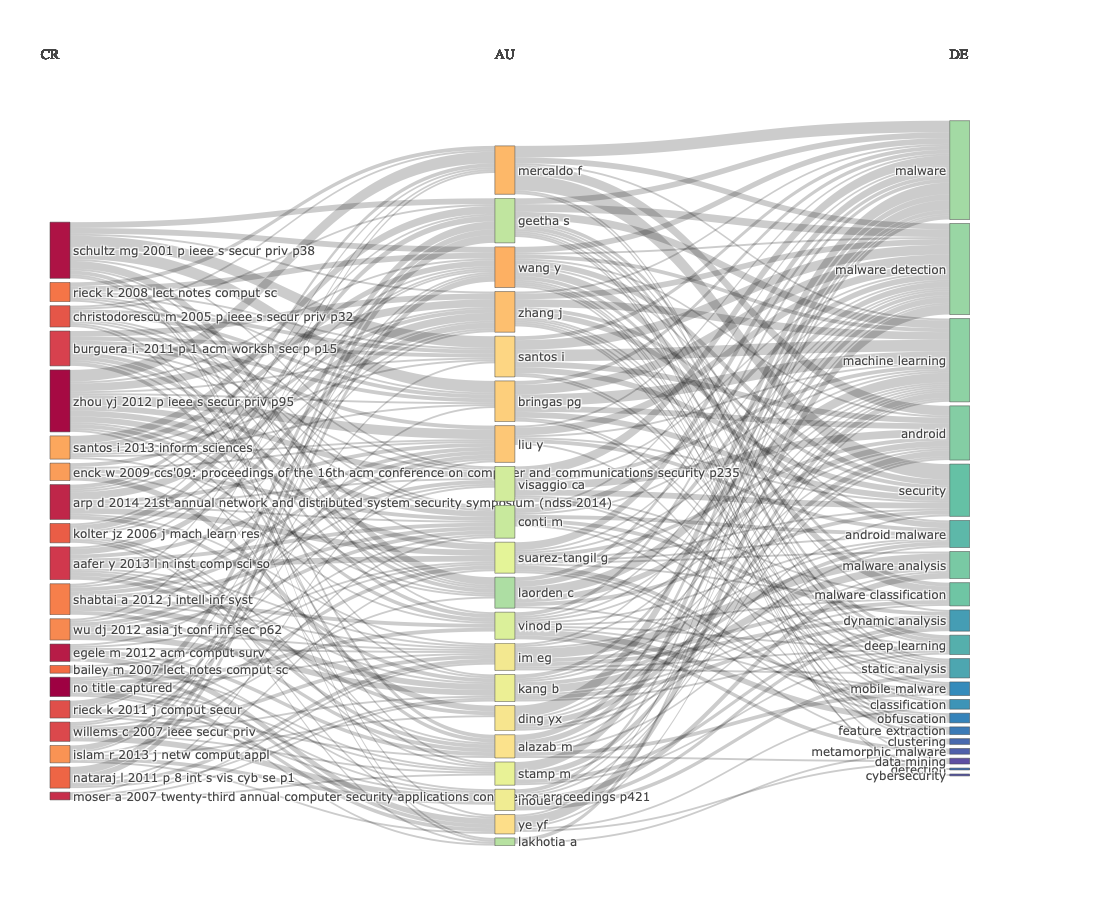
\includegraphics[width=1\textwidth]{experiments/gsmartins96/AnaliseBibliometrica/Malware/Figs/three_fields_plots.png}
    \caption{Plotagem ``Três Campos'' (Sankey plot) do \textit{dataset}: 20 Autores, Citações e Palavras-Chave mais proeminentes.}
    \label{fig:MALWARES@gsmartins96:ThreeFieldPlot}
\end{figure}

A figura \ref{fig:MALWARES@gsmartins96:ThreeFieldPlot} apresenta a plotagem do tipo ``Três Campos'' realizada no \textit{dataset}, vinculando à esquerda, as 20 Citações mais frequentes (CR - Cited Records), ao centro os 20 Autores mais proeminentes (AU), e à direita as 20 Palavras-Chave mais utilizadas pelos autores.
